%
% $Autor: Vikas Ramaswamy$
% $Datum: 2020-01-18 11:15:45Z $
% $Project: Pnuemonia detection $
% $Version: 1$
%
%
% !TeX encoding = utf8
% bibtex
%
%%%%%%




\Mysection{Introduction}
\STANDARD{Introduction to A Philosophy of Software Design}  
{
  \begin{itemize}
    \item A Philosophy of Software Design is a book by John Ousterhout that presents a set of principles and practices for designing high-quality software. Ousterhout is a well-known computer scientist and software engineer who has made significant contributions to the development of various programming languages and software systems.\newline
  
    \item The book argues that software design is more about understanding the problem domain than about implementing solutions. It emphasizes the importance of simplicity, clarity, and maintainability in software design, and provides practical guidance on how to achieve these goals.
   
   %\usepackage{tikz}
   %\usepackage{graphicx}

\begin{figure}
	\centering
	\begin{tikzpicture}
		\node at (0,0) {\includegraphics[width=4cm]{Images/1}};
	\end{tikzpicture}
	\caption{\textbf{Cover Page \cite{Ousterhout:2018}}}
	\label{fig:Cover Page}
\end{figure}

  \end{itemize}
}

\STANDARD{Introduction to Code Should be Obvious}
{ 

    
 According to "A Philosophy of Software Design" by John Ousterhout, for code to be obvious, it should be easy to understand and follow, even for someone who is not familiar with the codebase. The book argues that writing code that is self-documenting is key to achieving this goal. This means that the code should be written in a way that clearly communicates its purpose and behavior, with clear and concise names for functions, variables, and classes. \newpage
 
 The book provides several practical tips for making code obvious, including:\newline
    
   \begin{itemize}
    \item Use clear and descriptive names for variables, functions, and classes.
    Avoid overly complex code that is difficult to understand.
    Break down code into smaller, more manageable functions and modules.
   
    \item  Use comments and documentation sparingly, and only when necessary.
    Ensure that code is consistent in style and structure throughout the codebase.
    Avoid using overly clever or complex coding techniques that may be difficult to understand.  \newpage
     \item Overall, the book emphasizes the importance of simplicity, clarity, and maintainability in software design, and making code obvious is a key component of achieving these goals. By writing code that is easy to understand and follow, software engineers can reduce the likelihood of bugs and errors, improve the maintainability of the codebase, and ultimately deliver higher-quality software. \cite{Mancuso:2014}
   
  \end{itemize}

}
\Mysection{Importance for code}
\STANDARD{ Importance for code}
{ 

\begin{itemize}
	\item There are several reasons why it is important for code to be obvious. First, obvious code is easier to understand and maintain. This means that bugs can be fixed more quickly and new features can be added more easily. This can save time and money in the long run.
	
	\item Second, obvious code is more robust. When code is obvious, it is easier to test and debug. This means that it is less likely to contain bugs that could cause problems later on. Obvious code is also less likely to break when changes are made to it.
	
	\item Third, obvious code is more scalable. When code is obvious, it is easier to refactor and extend. This means that the code can be modified to meet changing requirements without causing problems elsewhere in the system. This can make it easier to add new features or modify existing ones.
	
\end{itemize}
}
\newpage 
\Mysection{How to achieve obvious code?}

\textbf{How to achieve obvious code?}\newline
{
\begin{itemize}
	
\item \textbf{Keep it simple}\newline
	 One of the key principles of good software design is to keep things simple. This means avoiding unnecessary complexity or abstraction. Simple code is easier to understand and maintain, and it is less likely to contain bugs.\newline
\item \textbf{Use meaningful names}\newline
	 Good variable names and function names can make a big difference in how easy code is to understand. Names should be descriptive and meaningful, and they should accurately reflect the purpose of the variable or function.\newline
\newpage
\item \textbf{Write clear comments}\newline
 Comments can be a powerful tool for making code more obvious. Good comments explain what the code does, why it is necessary, and how it works. Comments should be concise and clear, and they should not repeat the code.\newline
\item \textbf{Follow consistent coding conventions}\newline
Consistent coding conventions can make code easier to read and understand. This means using consistent indentation, formatting, and naming conventions. Consistent conventions can also make it easier to collaborate with other developers.\newline
\newpage
\item \textbf{Use modular design}\newline
Modular design is a key principle of good software design. This means breaking code down into smaller, more manageable components. Modular design can make code more obvious by reducing complexity and making it easier to understand.\cite{Zhou:2018} \newline

\end{itemize}


}
\Mysection{Example}

\STANDARD{Example}
{ 
	
	\begin{itemize}
		\item Let's consider an example of a function that calculates the factorial of a given number:\newline


\lstinputlisting[language=Python]{Code/factorial.py}

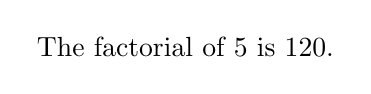
\begin{tikzpicture}
	% Set the value of n
	\def\n{5}
	
	% Calculate the factorial of n
	\pgfmathsetmacro\fact{int(\n*(\n>1)*(\n-1)*(\n-2)*(\n-3)*(\n-4))}
	
	% Draw the result
	\draw (0,0) node {The factorial of $\n$ is $\fact$.};
\end{tikzpicture} 

		The above implementation is recursive and it's quite obvious what it does. \newpage
		
		\item However, we can make it more obvious by using a loop:\newline
		
	\lstinputlisting[language=Python]{Code/factorial2.py}
		
		This implementation is more obvious because it's using a loop instead of recursion, which makes it easier to read and understand. The use of a loop also eliminates the risk of hitting the recursion limit for large values of n.\newline
		\newpage
		\item Furthermore, we can make it even more obvious by adding comments and meaningful variable names:\newline
	
	    	\lstinputlisting[language=Python]{Code/factorial1.py}
	
		
	\end{itemize}
}
\Mysection{Conclusion}
\STANDARD{Conclusion}
{
Code should be obvious is a key concept in good software design. Obvious code is easier to understand and maintain, more robust, and more scalable. Achieving obvious code requires a combination of good design principles and coding practices, including keeping things simple, using meaningful names, writing clear comments, following consistent coding conventions, and using modular design. By following these principles, developers can create software that is easier to understand, maintain, and extend.
}